\documentclass[10pt, aspectratio=169]{beamer}

% =========================
% THEME & COLORS — calmer palette
% =========================
\usetheme{Madrid}
\usecolortheme{default}

\definecolor{darkblue}{RGB}{0, 51, 102}
\definecolor{lightblue}{RGB}{224, 236, 248}
\definecolor{softblue}{RGB}{176, 198, 222}
\definecolor{boxfill}{RGB}{247, 250, 253}
\definecolor{softred}{RGB}{170, 86, 86}
\definecolor{softgreen}{RGB}{66, 126, 92}
\definecolor{softorange}{RGB}{180, 135, 62}
\definecolor{warmfill}{RGB}{250, 247, 242}
\definecolor{greenfill}{RGB}{243, 248, 245}
\definecolor{lightgray}{RGB}{245, 245, 245}
\definecolor{midgray}{RGB}{120, 120, 120}

\setbeamercolor{structure}{fg=darkblue}
\setbeamercolor{title}{fg=white, bg=darkblue}
\setbeamercolor{frametitle}{fg=darkblue, bg=lightblue}
\setbeamercolor{block title}{fg=white, bg=darkblue!82}
\setbeamercolor{block body}{bg=boxfill}
\setbeamercolor{block title alerted}{fg=white, bg=softred!88}
\setbeamercolor{block body alerted}{bg=warmfill}
\setbeamercolor{block title example}{fg=white, bg=softgreen!82}
\setbeamercolor{block body example}{bg=greenfill}

\setbeamertemplate{navigation symbols}{}
\setbeamertemplate{footline}{%
  \hfill\insertframenumber/\inserttotalframenumber\hspace{0.5cm}\vspace{0.3cm}
}

% =========================
% PACKAGES
% =========================
\usepackage[utf8]{inputenc}
\usepackage[T1]{fontenc}
\usepackage{lmodern}
\usepackage{amsmath,amssymb,amsthm}
\usepackage{graphicx}
\usepackage{booktabs}
\usepackage{tikz}
\usetikzlibrary{arrows.meta, positioning, calc, decorations.pathreplacing, shapes.geometric}
\usepackage{appendixnumberbeamer}
\usepackage{array}
\usepackage{ragged2e}
\usepackage{xcolor}

% =========================
% TITLE INFO
% =========================
\title[Horizontal Mergers \& Innovation]{\textbf{Horizontal Mergers and Innovation}}
\subtitle{Bruno Jullien \& Yassine Lefouili}
\author{Presented by\\ Tim K\"uhleis \and Muaz Ahmed \and Baptiste Vaux}
\institute{Paris School of Economics}
\date{24.03.2026}

% =========================
% MACROS
% =========================
\newcommand{\E}{\mathbb{E}}
\newcommand{\R}{\mathbb{R}}
\newcommand{\argmax}{\operatorname*{argmax}}
\newcommand{\argmin}{\operatorname*{argmin}}
\newcommand{\pos}[1]{\textcolor{softgreen}{#1}}
\newcommand{\negg}[1]{\textcolor{softred}{#1}}
\newcommand{\amb}[1]{\textcolor{softorange}{#1}}
\newcommand{\highlight}[1]{\textcolor{darkblue}{\textbf{#1}}}

\newcommand{\panelbox}[3][4.2cm]{%
  \fcolorbox{darkblue!18}{boxfill}{%
    \parbox[t][#1][t]{\linewidth}{%
      \textbf{#2}\par\vspace{0.35em}\small #3%
    }%
  }%
}

% =========================
% SECTION SLIDES
% =========================
\AtBeginSection[]{
  \begin{frame}
    \vfill
    \centering
    \begin{beamercolorbox}[sep=8pt,center,shadow=true,rounded=true]{title}
      \usebeamerfont{title}\insertsectionhead\par
    \end{beamercolorbox}
    \vfill
  \end{frame}
}

% =========================
% DOCUMENT
% =========================
\begin{document}

\begin{frame}
\titlepage
\end{frame}

% =========================
% OUTLINE
% =========================
\begin{frame}{Outline}
\tableofcontents
\end{frame}
% =========================================================
%  PART I — Setting the Stage - Policy Motivation and Framework
% =========================================================
% =========================================================
\section{Part I: Policy Motivation and Framework}
% =========================================================

% ----------------------------------------------------------
% SLIDE 1 — Introduction
% ----------------------------------------------------------
\begin{frame}{Introduction}
\small

\begin{itemize}
    \setlength{\itemsep}{0.5em}
    \item This presentation connects directly to recent sessions on innovation effects of mergers, in particular the FLV framework and last week's discussion of Denicolò \& Polo~(2018).
    \item Last week showed how the theoretical models laid out by the DG~Comp chief economist team \textit{(written in private capacity)} Federico, Langus \& Valletti~(2017, 2018) predict that mergers reduce innovation through internalization of what they call \highlight{cannibalization}. But also that this conclusion can be challenged.
    \item The paper we study today is a \highlight{comprehensive response}: it argues there is no basis for a general presumption that mergers harm innovation.
\end{itemize}

\vspace{0.4cm}

\begin{block}{Key Question}
Does economic theory support a presumption of harm, or is the effect of mergers on innovation inherently ambiguous?
\end{block}
\end{frame}

% ----------------------------------------------------------
% SLIDE 2 — From Pipeline Products to Innovation Spaces
% ----------------------------------------------------------
\begin{frame}{From Pipeline Products to Innovation Spaces}
\small

\begin{center}
\textit{Bunworth (2021) argues that competition law has become increasingly strict and interventionist in its treatment of innovation competition concerns.}
\end{center}

\vspace{0.5em}

\begin{center}
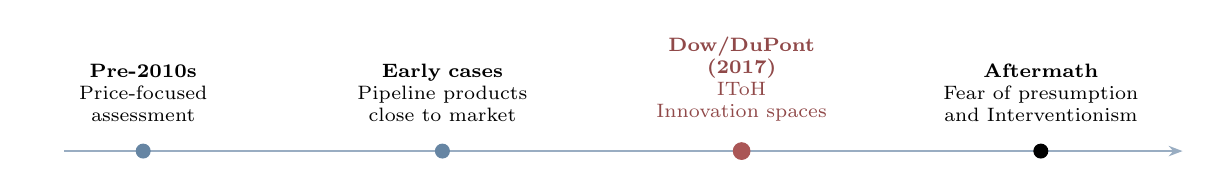
\begin{tikzpicture}[
    scale=1,
    every node/.style={font=\scriptsize},
    era/.style={text width=2.7cm, align=center},
]
  % Axis
  \draw[-{Stealth[length=5pt]}, thick, darkblue!40] (0,0) -- (14.2,0);

  % Era 1
  \filldraw[darkblue!60] (1.0,0) circle (2.5pt);
  \node[era, above=0.25cm] at (1.0,0) {\textbf{Pre-2010s}\\Price-focused assessment};

  % Era 2
  \filldraw[darkblue!60] (4.8,0) circle (2.5pt);
  \node[era, above=0.25cm] at (4.8,0) {\textbf{Early cases}\\Pipeline products\\close to market};

  % Era 3
  \filldraw[softred] (8.6,0) circle (3pt);
  \node[era, above=0.25cm, text=softred!85!black] at (8.6,0)
    {\textbf{Dow/DuPont (2017)}\\IToH\\Innovation spaces};

  % Era 4
  \filldraw[black] (12.4,0) circle (2.5pt);
  \node[era, above=0.25cm] at (12.4,0) {\textbf{Aftermath}\\Fear of presumption\\and Interventionism};
\end{tikzpicture}
\end{center}

\vspace{0.7em}

\begin{alertblock}{Dow/DuPont: innovation theory of harm}
\footnotesize
The intellectual backdrop was provided by FLV (2017, 2018): a merger may reduce R\&D because the merged firm internalizes business-stealing between its own innovation projects.

\vspace{0.3em}
In \textit{Dow/DuPont}, this logic was extended beyond \textbf{pipeline products} to \textbf{innovation spaces}: broad areas of R\&D aimed at future products or technologies with overlapping expected applications, even when no specific overlapping product is yet identifiable.
\end{alertblock}

\end{frame}

% ----------------------------------------------------------
% SLIDE 3 — The Presumption Debate (Bunworth)
% ----------------------------------------------------------
\begin{frame}{The Presumption Debate (Bunworth, 2021)}
\small

\begin{block}{Context}
Under Commissioner Vestager (2014--2024), DG~Comp pursued a broadly interventionist enforcement stance. Valletti himself proposed that innovative firms in tech should be required to \textit{affirmatively demonstrate} how acquisitions benefit consumers. Many practitioners feared a de facto presumption of harm was forming.
\end{block}

\vspace{0.3em}
\begin{columns}[T,onlytextwidth]
\begin{column}{0.47\textwidth}

\textbf{\negg{Arguments for presumption}}
\begin{itemize}
    \setlength{\itemsep}{0.3em}
    \item Innovation harm harder to measure than price increases no clear measurable object
    \item Information asymmetry favours defendants (more data to disprove harm)
    \item Kwoka (2020): policy debate overweighs Type~I errors (blocking good mergers) vs.\ Type~II (clearing harmful ones)
\end{itemize}

\end{column}
\begin{column}{0.47\textwidth}

\textbf{\pos{Arguments against presumption}}
\begin{itemize}
    \setlength{\itemsep}{0.3em}
    \item No consensus in econ literature on negative causal link
    \item Innovation $\neq$ pricing: fundamentally different economic problems
    \item R\&D is stochastic inputs $\neq$ outputs; research diversity is not a goal per se
    \item Commission rarely accepts efficiency defences asymmetric treatment of pro- and anti-competitive effects
\end{itemize}

\end{column}
\end{columns}

\vspace{0.3em}
{\footnotesize \textit{Note:} \S\,38 of the EU Horizontal Merger Guidelines itself acknowledges that mergers \textbf{can increase} firms' ability and incentive to innovate.}
\end{frame}


% ----------------------------------------------------------
% SLIDE 4 — Incentives vs. Ability
% ----------------------------------------------------------
\begin{frame}{Incentives vs.\ Ability to Innovate}
\small

\begin{columns}[T,onlytextwidth]
\begin{column}{0.48\textwidth}
\begin{block}{Incentives to Innovate}
How a merger changes firms' \textbf{strategic incentives to innovate}, holding organisation, technology, and capabilities fixed.

\vspace{0.35em}
\textit{Analogy:} unilateral effects in price analysis.
\end{block}
\end{column}

\begin{column}{0.48\textwidth}
\begin{block}{Ability to Innovate}
How a merger changes firms' \textbf{capacity to innovate}, for example through pooling R\&D assets, coordinating research activities, or exploiting complementarities.

\vspace{0.35em}
\textit{Analogy:} efficiencies in standard merger analysis.
\end{block}
\end{column}
\end{columns}

\vspace{0.6em}

\begin{center}
\parbox{0.9\textwidth}{\centering
\small
\textbf{Standard merger analysis for price concerns already follows this logic:} authorities typically assess \highlight{incentives} first, holding capabilities fixed, and then turn to \highlight{ability} effects such as efficiencies. We focus here on the incentives margin.
}
\end{center}

\end{frame}



% ----------------------------------------------------------
% SLIDE 5 — Why the FLV Framing Is Incomplete
% ----------------------------------------------------------
\begin{frame}{Limits of the FLV Framing}
\small

\begin{columns}[T,onlytextwidth]
\begin{column}{0.44\textwidth}

\textbf{1.\ Innovation externality}

\vspace{0.4em}
Post-merger, the firm internalizes business-stealing across its own R\&D efforts.

\vspace{0.4em}
$\Longrightarrow$ \negg{Lower innovation incentives}

\vspace{0.2em}
{\footnotesize Strongest when merging firms are close innovation rivals.}

\end{column}

\hfill
{\color{darkblue!25}\vrule width 0.4pt}
\hfill

\begin{column}{0.44\textwidth}

\textbf{2.\ Price coordination effect}

\vspace{0.4em}
A merger raises post-merger margins, increasing the payoff from successful R\&D.

\vspace{0.4em}
$\Longrightarrow$ \amb{Ambiguous effect}

\vspace{0.2em}
{\footnotesize Higher returns may or may not outweigh weaker competitive pressure.}

\end{column}
\end{columns}

\vspace{1.2em}

\begin{center}
\textbf{Standard implication in FLV-type models:}

\vspace{0.5em}
\[
\underbrace{\text{Innovation externality}}_{\text{large, negative}}
\;>\;
\underbrace{\text{Price coordination}}_{\text{ambiguous}}
\qquad\Longrightarrow\qquad
{\color{red!75!black}\Delta I < 0}
\]
\end{center}

\vspace{0.8em}

\begin{alertblock}{Jullien \& Lefouili's Critique}
This captures only \textbf{part of the incentives story}. Channels the FLV framework abstracts from demand expansion, technological spillovers, and the type of innovation can offset or dominate the negative effect.
\end{alertblock}

\end{frame}
% ----------------------------------------------------------
% SLIDE 6 — The Four-Term Decomposition + Thesis
% ----------------------------------------------------------
\begin{frame}{The Paper's Framework: A Four-Term Decomposition}
\small

Following Bourreau, Jullien \& Lefouili (2018), the total effect of a merger on innovation can be decomposed into \highlight{four distinct terms}:

\vspace{0.5em}
\[
\Delta I
=
\underbrace{\text{Innovation Diversion}}_{\text{\color{orange}$\pm$}}
+
\underbrace{\text{Demand Expansion}}_{\text{\color{green!60!black}+}}
+
\underbrace{\text{Margin Expansion}}_{\text{\color{red}-}}
+
\underbrace{\text{Interaction Term}}_{\text{\color{orange}?}}
\]

\vspace{0.3em}
\begin{columns}[T,onlytextwidth]
\begin{column}{0.47\textwidth}

\begin{itemize}
    \setlength{\itemsep}{0.3em}
    \item \textbf{Innovation diversion} {\footnotesize (\amb{$\pm$})}: internalization of sales externality; sign depends on type of innovation (vertical vs.\ horizontal)
    \item \textbf{Demand expansion} {\footnotesize (\pos{$+$})}: higher post-merger margins raise the return on demand-enhancing innovation
\end{itemize}

\end{column}
\begin{column}{0.47\textwidth}

\begin{itemize}
    \setlength{\itemsep}{0.3em}
    \item \textbf{Margin expansion} {\footnotesize (\negg{$-$})}: lower post-merger output reduces the scale over which margin improvements apply
    \item \textbf{Interaction term} {\footnotesize (\amb{$?$})}: joint determination of prices and innovation; cannot be signed a priori
\end{itemize}

\end{column}
\end{columns}

\vspace{0.35em}
\begin{exampleblock}{Jullien \& Lefouili's Thesis}
There should be \textbf{no general presumption} that mergers harm innovation. Instead, the authors call for a \highlight{case-by-case} assessment based on this decomposition, since focusing on one channel alone especially innovation diversion can be misleading.
\end{exampleblock}

\end{frame}
% =========================================================
%  PART II — THE CORE EFFECTS
% =========================================================
\section{Part II: The Core Effects and Theory}


% ----------------------------------------------------------
% SLIDE 2 — FLV Benchmark
% ----------------------------------------------------------
\begin{frame}{The Innovation Diversion Effect}
\small
\begin{block}{Core Idea}
A direct application of the classic \highlight{business-stealing externality} to innovation incentives. A merged entity internalizes cannibalization, lowering its incentives to innovate.
\end{block}
\vspace{0.2em}
\begin{columns}[T,onlytextwidth]
\begin{column}{0.6\textwidth}
\textbf{Illustrative Example}
\begin{itemize}
    \setlength{\itemsep}{0.15em}
    \item Incumbent(s) and a potential entrant that must innovate to enter.
    \item Successful entry \highlight{diverts sales} from incumbents.
    \item \textbf{Without merger:} R\&D decision depends only on own probability of success, expected profit, and costs.
    \item \textbf{With merger:} internalization of cannibalization $\Rightarrow$ lower incentives to innovate.
\end{itemize}
\vspace{0.3em}
{\footnotesize\textit{Formalized by FLV (2017): $N$ identical labs competing for a new market.}}
\end{column}
\begin{column}{0.40\textwidth}
\centering
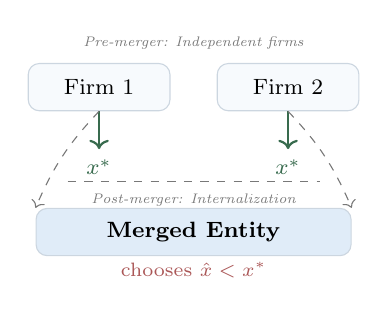
\begin{tikzpicture}[scale=0.8, every node/.style={font=\footnotesize}]
% Pre-merger
\node[font=\tiny\itshape, text=midgray] at (1.5,3.8) {Pre-merger: Independent firms};
\node[draw=darkblue!20, rounded corners, fill=boxfill, minimum width=1.8cm, minimum height=0.6cm] (L1) at (0,3.1) {Firm 1};
\node[draw=darkblue!20, rounded corners, fill=boxfill, minimum width=1.8cm, minimum height=0.6cm] (L2) at (3.0,3.1) {Firm 2};
\draw[->, thick, softgreen!85!black] (L1.south) -- ++(0,-0.6) node[below] {$x^*$};
\draw[->, thick, softgreen!85!black] (L2.south) -- ++(0,-0.6) node[below] {$x^*$};
% Divider
\draw[dashed, midgray, thin] (-0.5,1.6) -- (3.5,1.6);
% Post-merger
\node[draw=darkblue!20, rounded corners, fill=lightblue, minimum width=4cm, minimum height=0.6cm] (M) at (1.5,0.8) {\textbf{Merged Entity}};
\node[font=\tiny\itshape, text=midgray] at (1.5,1.3) {Post-merger: Internalization};
\draw[->, dashed, midgray] (L1.south) to[bend right=10] (M.north west);
\draw[->, dashed, midgray] (L2.south) to[bend left=10] (M.north east);
\node[text=softred, font=\scriptsize] at (1.5,0.2) {chooses $\hat{x} < x^*$};
\end{tikzpicture}
\end{column}
\end{columns}
\vspace{0.7em}
{\footnotesize\textit{\textbf{Note:} Jullien \& Lefouili \textbf{do not reject this mechanism}---their point is that it is only \highlight{one channel}, so it cannot by itself justify a general presumption of harm.}}
\end{frame}

% ----------------------------------------------------------
% SLIDE 3 — Why Diversion Isn't the Whole Story
% ----------------------------------------------------------

\begin{frame}{Why Diversion Is Not the Whole Story}
\small
\begin{block}{Core idea}
Counterarguments to the claim that merger-induced innovation diversion must \emph{strictly reduce} R\&D incentives.
\end{block}

\vspace{0.2em} 

\begin{columns}[T,onlytextwidth]
    \hfill % Adds flexible space on the left
    \begin{column}{0.31\textwidth} % Slightly reduced width to ensure fit
    \panelbox[2.8cm]{1. Focus \& Intensity}{
    Mergers can shut one path to \emph{intensify} effort on another.\\[0.35em]
    {\footnotesize \textbf{Denicolò \& Polo (2018):} Concentration can \pos{raise} innovation probability.}
    }
    \end{column}
    \hfill % Adds flexible space between box 1 and 2
    \begin{column}{0.31\textwidth}
    \panelbox[2.8cm]{2. Innovation Type}{
    \textbf{Vertical:} Diversion effect \negg{negative} (quality jumps steal rival demand).\\[0.35em]
    \textbf{Horizontal:} Diversion effect \pos{positive} (softens price competition).
    }
    \end{column}
    \hfill % Adds flexible space between box 2 and 3
    \begin{column}{0.31\textwidth}
    \panelbox[2.8cm]{3. Pricing Strategy}{
    Merged firms \emph{adjust prices} to mitigate cannibalization.\\[0.35em]
    {\footnotesize \textbf{Jullien \& Lefouili (2018):} Incremental profits may actually increase.}
    }
    \end{column}
    \hfill % Adds flexible space on the right
\end{columns}

\vspace{0.5em}
\centering
\itshape\color{darkblue!70!black}
$\Downarrow$\quad conclusion \quad$\Downarrow$
\smallskip

\fcolorbox{darkblue!50}{darkblue!8}{\parbox{0.9\linewidth}{
\centering\bfseries
Diversion is a valid channel, but it does \emph{not} imply a systematic decline in post-merger innovation.
}}
\end{frame}


% ----------------------------------------------------------
% SLIDE 4 — Demand Expansion
% ----------------------------------------------------------
\begin{frame}{Demand Expansion: Higher Margins Can Spur Innovation}
\small
\begin{block}{\small Setting (Bourreau, Jullien \& Lefouili, 2018)}
\footnotesize Innovation mainly \highlight{expands demand} w/o significantly affecting the margin. Return to R\&D depends on the profit earned on each additional unit sold.
\end{block}
\vspace{0.15em}
\[
\Pi^{\text{innov}} \;=\; \underbrace{M_0}_{\text{\scriptsize margin}}\;\bigl(\underbrace{Q_1(X)-Q_0}_{\text{\scriptsize demand expansion}}\bigr)\;-\;X
\]
\vspace{0.1em}
\begin{itemize}\setlength{\itemsep}{0.2em}
  \item $M_0$ acts as a \textbf{multiplier} on the demand gain --- key trade-off: margin vs.\ sales, governed by own-price elasticity
  \item \textbf{Chain:} Merger relaxes price competition $\to$ $M_0$ \pos{rises} $\to$ each extra unit of demand worth more $\to$ \pos{higher R\&D incentive}
  \item First shown for telecom coverage (Bourreau \& Jullien, 2018), generalized in Bourreau, Jullien \& Lefouili (2018)
\end{itemize}
\vspace{0.15em}
$\Rightarrow$ \textbf{Positive channel}: relaxed price competition raises margins, increasing the payoff from demand-enhancing innovations.
\end{frame}

\begin{frame}{Telecom Coverage: An Illustration of Demand Expansion}
\small

% --- TIER 1: POLICY CONTEXT ---
\begin{beamercolorbox}[sep=4pt, rounded=true, shadow=false]{block body}
    \scriptsize
    \textbf{Context:} EU mobile mergers spark debate: Operators claim they foster new tech (4G/5G), while the EC fears reduced investment incentives \par \vspace{0.2em}
    $\rightarrow$ \highlight{BJ (2018):} A simultaneous \textbf{coverage-price game} where firms decide on coverage ($x$) and a single uniform price across all zones
\end{beamercolorbox}

\vspace{0.4cm}

% --- TIER 2: THE VISUAL MODEL ---
\centering
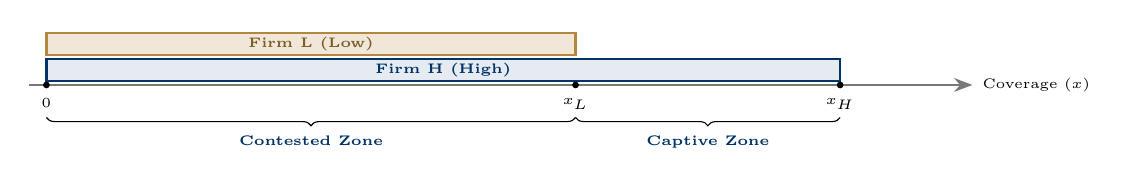
\begin{tikzpicture}[x=11.2cm, y=0.55cm, every node/.style={font=\scriptsize}]
    % Axis
    \draw[thick, -{Stealth}, midgray] (-0.02,0) -- (1.05,0) node[right, black] {\tiny Coverage ($x$)};
    
    % Coverage Bars
    \fill[softorange!20, draw=softorange, thick] (0,0.7) rectangle (0.6,1.2) 
        node[pos=.5, softorange!70!black, font=\bfseries\tiny] {Firm L (Low)};
    \fill[darkblue!10, draw=darkblue, thick] (0,0.1) rectangle (0.9,0.6) 
        node[pos=.5, darkblue, font=\bfseries\tiny] {Firm H (High)};

    % Coordinates
    \foreach \x/\lab in {0/0, 0.6/x_L, 0.9/x_H}
        {\filldraw (\x,0) circle (1pt); \node[below=1.5pt] at (\x,0) {\tiny $\lab$};}

    % Labels for Zones
    \draw [decorate, decoration={brace, amplitude=3pt, mirror}] (0,-0.75) -- (0.6,-0.75) 
        node [midway, below=3pt, align=center] {\highlight{\tiny Contested Zone}};
        
    \draw [decorate, decoration={brace, amplitude=3pt, mirror}] (0.6,-0.75) -- (0.9,-0.75) 
        node [midway, below=3pt, align=center] {\highlight{\tiny Captive Zone}};
\end{tikzpicture}

\vspace{0.4cm}

% --- TIER 3: PRE- VS POST-MERGER COMPARISON ---
\begin{columns}[T,onlytextwidth]
    \begin{column}{0.48\textwidth}
        \textbf{\textcolor{darkblue}{Pre-Merger (Duopoly)}}
        \vspace{-0.05cm} % Subtly reduces the default gap for a "normal" look
        \begin{itemize}
            \item[\tiny$\bullet$] Large contested share \textbf{forces prices down}
            \item[\tiny$\bullet$] \textbf{Low Margins} $\rightarrow$ Low ROI for expansion
        \end{itemize}
    \end{column}

    \begin{column}{0.48\textwidth}
        \textbf{\textcolor{darkblue}{Post-Merger (Monopoly)}}
        \vspace{-0.05cm} % Subtly reduces the default gap for a "normal" look
        \begin{itemize}
            \item[\tiny$\bullet$] Prices rise toward monopoly levels
            \item[\tiny$\bullet$] \textbf{High Margins} $\rightarrow$ High ROI for \textbf{Expansion}
        \end{itemize}
    \end{column}
\end{columns}

\vspace{0.6cm}

% --- TIER 4: SUMMARY ---
\centering
\begin{minipage}{0.9\textwidth}
    \centering
    \textbf{Consumer Welfare ($\Delta CS$):} 
    \negg{Price $\uparrow$} $+$ \negg{Variety $\downarrow$} $+$ \pos{Coverage $\uparrow\uparrow$} \\
    \vspace{0.2em}
    \textit{\footnotesize If the expansion into unserved areas is large, a merger increases total welfare.}
\end{minipage}

\end{frame}


% ----------------------------------------------------------
% SLIDE 5 — Margin Expansion
% ----------------------------------------------------------
\begin{frame}{Margin Expansion: Lower Output Weakens Innovation Incentives}
\small
\begin{block}{\small Setting (Bourreau, Jullien \& Lefouili, 2018)}
\footnotesize Innovation mainly raises the \highlight{margin per unit} w/o significantly expanding demand. Return to R\&D depends on how many units the margin gain applies to.
\end{block}
\vspace{0.15em}
\[
\Pi^{\text{innov}} \;=\; \bigl(\underbrace{M_1(X)-M_0}_{\text{\scriptsize margin gain}}\bigr)\;\cdot\;\underbrace{Q_0}_{\text{\scriptsize output}}\;-\;X
\]
\vspace{0.1em}
\begin{itemize}\setlength{\itemsep}{0.2em}
  \item $Q_0$ acts as a \textbf{multiplier} on the margin gain --- w/o efficiency gains, merger raises prices and lowers pre-innovation output
  \item \textbf{Chain:} Merger $\to$ price coordination $\to$ $Q_0$ \negg{falls} $\to$ margin gains apply to fewer units $\to$ \negg{lower R\&D incentive}
  \item Analog for \textbf{process innovation}: benefit of cost reduction is larger at higher output (Motta \& Tarantino, 2018)
\end{itemize}
\vspace{0.15em}
$\Rightarrow$ Main \textbf{negative channel}. Drives negative results in FLV (2018) and Motta \& Tarantino (2018), where demand specifications make this effect dominate by construction.
\end{frame}

% ----------------------------------------------------------
% SLIDE 6 — Model artifacts
% ----------------------------------------------------------
\begin{frame}{Why Some Models Systematically Deliver Negative Results}
\small

\begin{block}{The authors' claim}
Negative merger results in parts of the literature are not general economic theorems. They often arise because the demand specification imposes simplifying restrictions that \textit{mechanically} generate a negative sign.
\end{block}

\vspace{0.7em}

\textbf{How specific structures force negative results:}
\vspace{0.3em}
\begin{itemize}
    \setlength\itemsep{0.65em}
    \item \textbf{Hedonic prices:} Demand expansion and diversion offset each other, leaving the negative margin expansion effect to dominate.
    \item \textbf{Quality-adjusted demand:} Similar to hedonic prices, the specification inherently restricts the way innovation affects demand.
    \item \textbf{CES demand (FLV):} The mathematical structure guarantees the sum of terms is negative, independent of broader market features.
\end{itemize}

\vspace{0.9em}
$\Rightarrow$ If negative results rely on modeling shortcuts introduced for tractability, they cannot justify a general policy rule. This weakens the case for a \textbf{presumption} of harm.

\end{frame}

% ----------------------------------------------------------
% SLIDE 7 — Counterexample
% ----------------------------------------------------------

\begin{frame}{Counterexample: Hotelling with Horizontal Innovation}
\small

\textbf{Bourreau, Jullien \& Lefouili (2018)} consider a Hotelling model where innovation is \highlight{horizontal}---it increases product differentiation rather than quality.

\vspace{0.3em}
\begin{columns}[T,onlytextwidth]
\begin{column}{0.50\textwidth}

\textbf{Why the Merger increases Incentives to innovate:}
\begin{itemize}\setlength\itemsep{0.3em}
  \item Greater differentiation \textbf{relaxes price competition}
  \item Business stealing weakens $\Rightarrow$ diversion turns \pos{positive}
  \item Demand expansion also \pos{positive}
  \item These dominate the \negg{negative} margin expansion
\end{itemize}

\vspace{0.3em}
{\footnotesize \textbf{Note:} \textit{Holds even in a merger to monopoly, with no spillovers or efficiencies.}}

\end{column}
\begin{column}{0.46\textwidth}
\centering
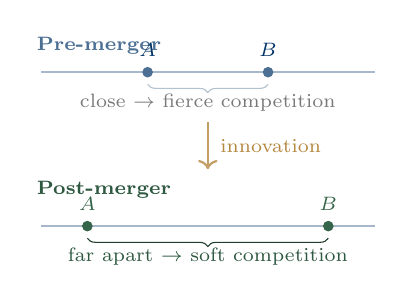
\begin{tikzpicture}[scale=0.85, every node/.style={font=\small}]
  %% PRE-MERGER
  \node[font=\scriptsize\bfseries, darkblue!70, anchor=west] at (-0.2, 0.4) {Pre-merger};
  \draw[thick, darkblue!35] (0,0) -- (5,0);
  \filldraw[darkblue!70] (1.6,0) circle (2pt)
    node[above=2pt, font=\scriptsize, darkblue] {$A$};
  \filldraw[darkblue!70] (3.4,0) circle (2pt)
    node[above=2pt, font=\scriptsize, darkblue] {$B$};
  \draw[decorate, decoration={brace, mirror, amplitude=3pt}, darkblue!30]
    (1.6,-0.18) -- (3.4,-0.18);
  \node[font=\scriptsize, midgray] at (2.5,-0.45) {close $\to$ fierce competition};

  %% Arrow - Adjusted to bridge the gap
  \draw[->, thick, softorange!80] (2.5,-0.75) -- (2.5,-1.45);
  \node[font=\scriptsize, softorange, right=1pt] at (2.5,-1.1) {innovation};

  %% POST-MERGER
  \node[font=\scriptsize\bfseries, softgreen!70!black, anchor=west] at (-0.2,-1.75) {Post-merger};
  
  \draw[thick, darkblue!35] (0,-2.30) -- (5,-2.30);
  \filldraw[softgreen!80!black] (0.7,-2.30) circle (2pt)
    node[above=2pt, font=\scriptsize, softgreen!80!black] {$A$};
  \filldraw[softgreen!80!black] (4.3,-2.30) circle (2pt)
    node[above=2pt, font=\scriptsize, softgreen!80!black] {$B$};
    
  \draw[decorate, decoration={brace, mirror, amplitude=3pt}, softgreen!50!black]
    (0.7,-2.48) -- (4.3,-2.48);
  \node[font=\scriptsize, softgreen!70!black] at (2.5,-2.75)
    {far apart $\to$ soft competition};
\end{tikzpicture}
\end{column}
\end{columns}

\vspace{0.3em}
\begin{alertblock}{Implication}
Even absent spillovers or efficiencies, a merger can \pos{increase} innovation---enough to reject a general presumption that horizontal mergers reduce product innovation.
\end{alertblock}
\end{frame}

% ----------------------------------------------------------
% SLIDE 8 — Synthesis
% ----------------------------------------------------------
\begin{frame}{Synthesis: Decomposing Merger Effects on Innovation}
\small

\begin{center}
\footnotesize
$
\Delta I = 
\underbrace{\text{Innov. diversion}}_{\textcolor{orange!80}{\pm}} +
\underbrace{\text{Demand expansion}}_{\textcolor{green!60!black}{+}} +
\underbrace{\text{Margin expansion}}_{\textcolor{red!70}{-}} +
\underbrace{\text{Interaction term}}_{\textcolor{orange!80}{?}}
$
\end{center}

\vspace{0.8em}
\begin{columns}[T,onlytextwidth]
\begin{column}{0.46\textwidth}

\textbf{What authorities should do:}
\begin{enumerate}
  \item evaluate \textbf{all four channels}, not just diversion;
  \item classify the \textbf{type of innovation} (vertical vs. horizontal);
  \item map effects on demand, margins, and differentiation;
  \item account for post-merger pricing adjustments.
\end{enumerate}

\end{column}
\begin{column}{0.46\textwidth}

\textbf{Additional Considerations in Part III:}
\begin{itemize}
  \item technological \highlight{spillovers};
  \item R\&D \highlight{complementarities};
  \item \highlight{process innovation}, where the negative channel is clearest.
\end{itemize}

\end{column}
\end{columns}

\vspace{0.9em}
\centering
\fcolorbox{darkblue!18}{boxfill}{\parbox{0.77\linewidth}{\centering
\textbf{The effect on innovation is a balancing problem, not a presumption problem.}
}}
\end{frame}


% =========================================================
%  PART III — Extending the Framework: Spillovers,
%             Complementarities & Policy
% =========================================================
\section{Part III: Spillovers, Complementarities \& Policy}


%% ============================================================
%% SLIDE 28 — Technological Spillovers
%% ============================================================
\begin{frame}{Technological Spillovers — A Countervailing Force}
  \begin{itemize}
    \item R\&D generates knowledge that spills over to rivals
          through patent disclosures, researcher mobility,
          and sequential innovation.

    \item Pre-merger, firms restrict knowledge sharing to prevent rivals from benefiting. Post-merger, the motive for exclusion vanishes, actively \textbf{increasing} the volume of spillovers between the partners.
    
  \end{itemize}

  \medskip
  \centering
  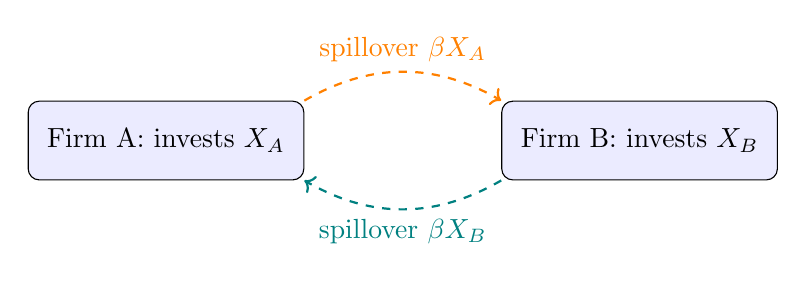
\begin{tikzpicture}
    \node[draw, rounded corners, fill=blue!8, 
          minimum width=3.5cm, minimum height=1cm] (A) 
          {Firm A: invests $X_A$};
    \node[draw, rounded corners, fill=blue!8, 
          minimum width=3.5cm, minimum height=1cm,
          right=2.5cm of A] (B) 
          {Firm B: invests $X_B$};
    \draw[->, thick, dashed, orange] 
          (A.north east) to[bend left=30] 
          node[above] {spillover $\beta X_A$} (B.north west);
    \draw[->, thick, dashed, teal] 
          (B.south west) to[bend left=30] 
          node[below] {spillover $\beta X_B$} (A.south east);
  \end{tikzpicture}

  \begin{block}{Implication}
    Spillovers belong in the main competitive assessment,
    not as a secondary efficiency defence.
  \end{block}
\end{frame}


%% ============================================================
%% SLIDE 29 — Net Innovation Pressure
%% ============================================================
\begin{frame}{Formalising the Spillover–Diversion Trade-off}
  \begin{itemize}
    \item Two ratios matter: the \textbf{spillover ratio} $\beta$
          (knowledge leaking to rivals) and the
          \textbf{innovation diversion ratio} $\delta_I$
          (demand stolen from rivals).

    \item The merger raises innovation if and only if:
  \end{itemize}

  \[
    \underbrace{\beta}_{\text{spillover ratio}}
    \;>\;
    \underbrace{\delta_I}_{\text{diversion ratio}}
    \qquad \Longleftrightarrow \qquad
    \underbrace{(\beta - \delta_I)}_{\text{Net Innovation Pressure}} > 0
  \]

  \begin{itemize}
    \item This is a clean condition when price effects are set
          aside. With active price competition, the full
          four-term decomposition supplements it.
  \end{itemize}

  \begin{block}{Key Insight}
    NIP is the innovation analogue of UPP: a structured
    directional input, not a standalone screen.
  \end{block}
\end{frame}


%% ============================================================
%% SLIDE 30 — R&D Complementarities
%% ============================================================
\begin{frame}{R\&D Complementarities — Ability to Innovate}
  \begin{itemize}
    \item Mergers can expand the \textit{capacity} to innovate
          by pooling labs, researchers, and know-how.

    \item Pre-merger, firms are reluctant to share knowledge
          with rivals. Post-merger, this barrier disappears.

    \item Production efficiencies that prevent output
          contraction reduce the margin expansion effect
          and amplify the demand expansion effect:
  \end{itemize}

  \[
    \underbrace{c \downarrow}_{\text{efficiency gain}}
    \;\Rightarrow\;
    \underbrace{p \downarrow}_{\text{price falls}}
    \;\Rightarrow\;
    \underbrace{Q \uparrow}_{\text{output rises}}
    \;\Rightarrow\;
    \underbrace{\Delta I \uparrow}_{\text{innovation incentive rises}}
  \]

  \begin{block}{Takeaway}
    A price-effects efficiency defence may resolve the
    innovation concern at the same time. Evaluate jointly.
  \end{block}
\end{frame}


%% ============================================================
%% SLIDE 31 — Process Innovation (brief aside)
%% ============================================================
\begin{frame}{A Brief Note on Process Innovation}
  \begin{itemize}
    \item Process innovation reduces costs but does not 
          expand demand. Two terms of the decomposition 
          drop out:
  \end{itemize}

  \[
    \Delta I \;\propto\;
    \underbrace{-\,\alpha\,\Delta Q}_{\text{margin exp. }(-)}
    \;+\;
    \textcolor{gray}{\underbrace{\delta_P M_0}_{\text{demand exp. }= \,0}}
    \;-\;
    \underbrace{\delta_I M_0}_{\text{diversion }(-)}
    \;+\;
    \textcolor{gray}{\underbrace{\gamma \Delta P}_{\text{interaction }=\, 0}}
  \]

  \begin{itemize}
    \item The negative channel is clearest here.
    \item However, when investment decisions are observable before
      price-setting, each firm's R\&D signals
      aggressiveness to rivals, inducing restraint
      across the industry. The net merger effect
      becomes generally ambiguous even here.
  \end{itemize}


\end{frame}


%% ============================================================
%% SLIDE 32 — Policy Implications
%% ============================================================
\begin{frame}{Policy Implications — J\&L's Message to DG~Comp}
  \begin{itemize}
    \item \textbf{Reject the IToH as currently applied.}
          DG~Comp has not established causation between
          concentration and reduced innovation. Dow/DuPont
          cannot support a general presumption.

    \item \textbf{Move beyond structural shortcuts.} Firm
          count is one input, but a 5-to-4 reduction is not
          sufficient on its own to establish harm.

    \item \textbf{Apply the full balancing framework}:

  \end{itemize}

  \[
    \Delta I \;=\;
    \underbrace{\delta_I\text{-term}}_{\pm}
    \;+\;
    \underbrace{\text{demand exp.}}_{+}
    \;+\;
    \underbrace{\text{margin exp.}}_{-}
    \;+\;
    \underbrace{\text{interaction}}_{?}
    \;+\;
    \underbrace{\beta\text{-adjustment}}_{\pm}
  \]

  \begin{block}{Recipe}
    A sound assessment is a neutral balancing exercise
    across all channels
  \end{block}
\end{frame}


%% ============================================================
%% SLIDE 32b — Case Application: Dow/DuPont
%% ============================================================
\begin{frame}{Case Application — Dow/DuPont (2017)}

  \begin{columns}[T]
    \begin{column}{0.48\textwidth}
      \textbf{What DG~Comp assessed}
      \begin{itemize}
        \item 5 $\to$ 4 innovators in crop protection
        \item Focus on diversion: fewer labs 
              $\Rightarrow$ less innovation
        \item Remedies required divestiture 
              of R\&D assets
      \end{itemize}
    \end{column}
    \begin{column}{0.48\textwidth}
      \textbf{What the framework says was missing}
      \begin{itemize}
        \item $\beta > 0$: significant cross-firm 
              knowledge flows in agri-chemicals
        \item Demand expansion: higher margins 
              post-merger raise returns to 
              product innovation
        \item R\&D pooling: complementary 
              pipelines in seeds and chemicals
      \end{itemize}
    \end{column}
  \end{columns}

  \medskip
  \begin{alertblock}{Bottom Line}
    DG~Comp evaluated $\delta_I$ in isolation.
    A full assessment would require signing
    $(\beta - \delta_I)$ and weighing all four terms
    before concluding harm.
  \end{alertblock}
\end{frame}


%% ============================================================
%% SLIDE 33 — Disclaimer on Positioning
%% ============================================================
\begin{frame}{A Note on the Paper's Positioning}
  \begin{itemize}
    \item Funded by a major law firm and economic consultancy.
          The authors disclose this. Arguing against
          presumption when causation is unestablished
          is analytically standard.

    \item The paper is oriented towards policy practice aimed
          at DG~Comp. Positive channels
          get more formal treatment than negative ones.

    \item Calling for neutrality has asymmetric enforcement
          consequences. That does not make the argument wrong,
          but it is worth keeping in mind.
  \end{itemize}


\end{frame}


%% ============================================================
%% SLIDE 34 — Ambiguity as the Main Result
%% ============================================================
\begin{frame}{Ambiguity Is the Point}
  \begin{itemize}
    \item The central result is theoretical ambiguity.
      Since DG~Comp bears the burden of proof,
      this is sufficient to defeat the IToH
      on its own terms.
    \item This was the goal from the start: show that the
          causal chain from concentration to reduced
          innovation is not established in theory, and
          therefore cannot ground a general presumption.
    \item The open question is a feature of this paper.
          It is a challenge for the broader empirical
          literature: how do you measure the terms of
          the decomposition in actual cases?
  \end{itemize}
  \begin{alertblock}{Implication}
    The rebuttal of the IToH is complete on its own terms.
    What comes next belongs to the empirical agenda,
    not to this paper.
  \end{alertblock}
\end{frame}


%% ============================================================
%% SLIDE 35 — Empirical Gaps
%% ============================================================
\begin{frame}{An Open Research Agenda}
  \begin{itemize}
    \item The decomposition identifies what matters. Estimating
          $\delta_I$, $\beta$, $\Delta Q$, and the interaction
          term in real merger cases is a separate and
          largely unsolved empirical problem.
    \item This is a field-wide challenge, not a gap specific
          to this paper. The same measurement problem
          exists for UPP in price-effects analysis, and
          decades of work have gone into it.
    \item The natural next step is structural estimation of
          the decomposition terms using merger data, building
          on the same toolkit used for demand-side price
          analysis.
  \end{itemize}
  \begin{alertblock}{Takeaway}
    The theoretical debate was reintroduced. The empirical
    tools to further it are still being built.
  \end{alertblock}
\end{frame}


%% ============================================================
%% SLIDE 36 — Where the Theory Stands
%% ============================================================
\begin{frame}{Where the Theory Stands Today}
  \begin{itemize}
    \item The paper's core contribution is showing that
          innovation diversion is one channel among several.
          DG~Comp's Dow/DuPont reasoning did not weigh the
          offsetting forces and therefore did not establish
          causation.
    \item Subsequent work has identified further positive
          channels J\&L did not fully develop -- notably,
          post-merger access to each other's research
          outputs, which further complicates the picture
          and reinforces the case against a general
          presumption (Calanchi \& Peya, 2025).
  \end{itemize}
  \begin{block}{Takeaway}
    The literature has moved from a presumption of harm
    to a balanced, case-by-case view. J\&L were central
    to that shift.
  \end{block}
\end{frame}


%% ============================================================
%% SLIDE 37 — Where the Policy Stands
%% ============================================================
\begin{frame}{Where the Policy Stands Today}
  \begin{itemize}
    \item The broad IToH peaked at Dow/DuPont and
          Bayer/Monsanto in 2017--18 and has not been
          applied in that form in traditional sectors since.
    \item The ECJ's 2023 ruling in CK Telecoms sided with
          the Commission on standard of proof, so the
          retreat was not forced by courts. The Commission
          retained the legal tools but stopped using them.
    \item The Draghi Report, Ribera's mission letter, and
          the ongoing EU Merger Guidelines review provided the political
          cover for a less interventionist turn.
  \end{itemize}
  \begin{block}{Takeaway}
    The IToH did not fall to one argument.
    Theory changed the terms of the debate.
    Politics changed the outcome.
  \end{block}
\end{frame}


%==========================
% Literature 
%==========================
\appendix

\begin{frame}[allowframebreaks]{Literature}
    \footnotesize
    \setbeamertemplate{bibliography item}[text] % Uses [1] instead of icons
    \bibliographystyle{apalike}
    
    \nocite{*} % This is the "magic" line that pulls everything in automatically
    \bibliography{references} 
\end{frame}


% =========================
% APPENDIX
% =========================

\begin{frame}{Appendix: Formal Decomposition}
\small
In a symmetric duopoly (Bourreau, Jullien \& Lefouili 2018), the change in R\&D incentives from a merger decomposes into four terms.

\vspace{0.5em}
\[
\Delta \text{R\&D}
\;\propto\;
\underbrace{-\,\alpha\,\Delta Q}_{\text{Margin Expansion }\negg{(-)}}
\;+
\underbrace{\delta_P\,M_0}_{\text{Demand Expansion }\pos{(+)}}
\;-
\underbrace{\delta_I\,M_0}_{\text{Diversion }\amb{(\pm)}}
\;+
\underbrace{\gamma\,\Delta P}_{\text{Interaction }\amb{(?)}}
\]

\vspace{0.6em}
\renewcommand{\arraystretch}{1.28}
\begin{tabular}{>{\bfseries}l l}
\toprule
Symbol & Interpretation \\
\midrule
$\delta_P$ & Price diversion ratio: share of demand diverted when price falls \\
$\delta_I$ & Innovation diversion ratio: share of demand diverted when R\&D rises \\
$\Delta Q$ & Output reduction due to post-merger pricing \\
$\gamma$ & Change in the relative impact of innovation and price on demand \\
\bottomrule
\end{tabular}

\vspace{0.5em}
\textbf{Key insight:} in restrictive demand systems, positive and negative terms can cancel mechanically. In more flexible environments such as Hotelling, the positive forces may dominate.
\end{frame}

\end{document}
